\subsection{Kinematics}
\label{kinematics}

\label{EXP}
We propose to measure the tensor asymmetry $A_{zz}$ for $\XMIN<x<\XMAX$, $\QMIN$~(GeV/$c)^2 < Q^2 <\QMAX$~(GeV/$c)^2$, and $\WMIN < W_{NN} < \WMAX$~GeV and extract the tensor analyzing power $T_{20}$ for $\QMINT20$~(GeV/$c)^2 < Q^2 <\QMAXT20$~(GeV/$c)^2$. Central kinematics of the spectrometers are given in Table~\ref{RATES1}
%, estimates for the uncertainties of $A_{zz}$ are given in Tables~\ref{RATES2}-\ref{RATES3}, and estimates for the uncertainties of $T_{20}$ are given in Table\need
. Fig.~\ref{kincov} shows the planned kinematic coverage utilizing the Hall C HMS and SHMS spectrometers at forward angles. 

\begin{table}
\begin{center}
\begin{tabular}{cc|c|c|c|c|c|c}
 & & $E_0$ & $Q^2$    	& $E'$  &    $\theta_{e'}$  &  Rates   & PAC Time   \\
%& (GeV) & (GeV$^2$)  & (GeV)  &     (deg.)   &   (kHz)  & (hours) \\
& & (GeV) & (GeV$^2$)  & (GeV)  &     ($^{\circ}$)   &   (kHz)  & (Days) \\
%\multicolumn{2}{|c|}{$\times 10^{-2}$}
\hline\hline
SHMS & (S1) & 8.8	&  1.5	&  8.36	&    8.2  	&    0.38	&   25 \\
HMS  & (H1) & 8.8	&  2.9	&  7.26	&    12.2	&    0.04	&   25 \\  
SHMS & (S2) & 6.6	&  0.7	&  6.35	&    7.5 	&    3.57	&   8 \\
HMS  & (H2) & 6.6	&  1.8	&  5.96	&    12.3	&    0.09	&   8 \\  
SHMS & (S3) & 2.2	&  0.2	&  2.15	&    10.9 	&    10.5	&   1 \\
HMS  & (H3) & 2.2	&  0.3	&  2.11	&    14.9	&    3.23	&   1 \\  
\hline\hline
\end{tabular}
\caption{\label{RATES1}Summary of the central kinematics and physics rates using the Hall C  spectrometers.}
\end{center}
\end{table}









\begin{figure}
\begin{center}
%\includegraphics[width=\textwidth]{figs/Pzz_30_all_q2_w.eps}
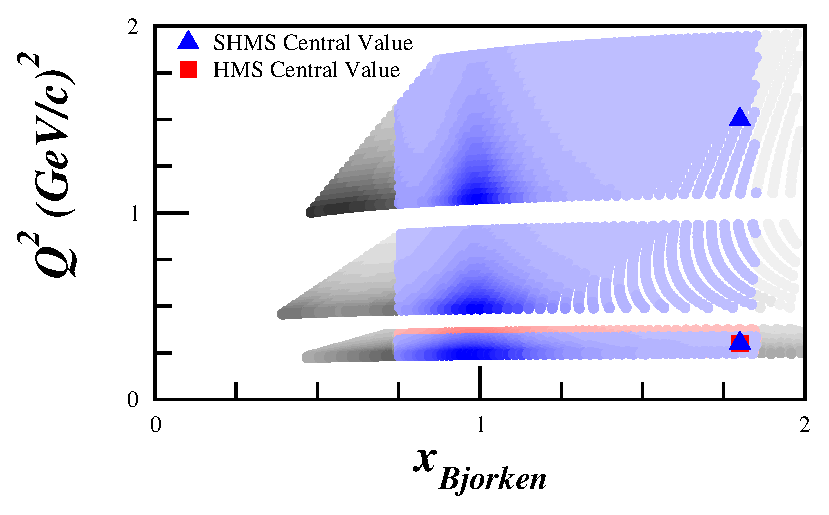
\includegraphics[width=0.49\textwidth]{figs/Pzz_30_all_q2.eps}

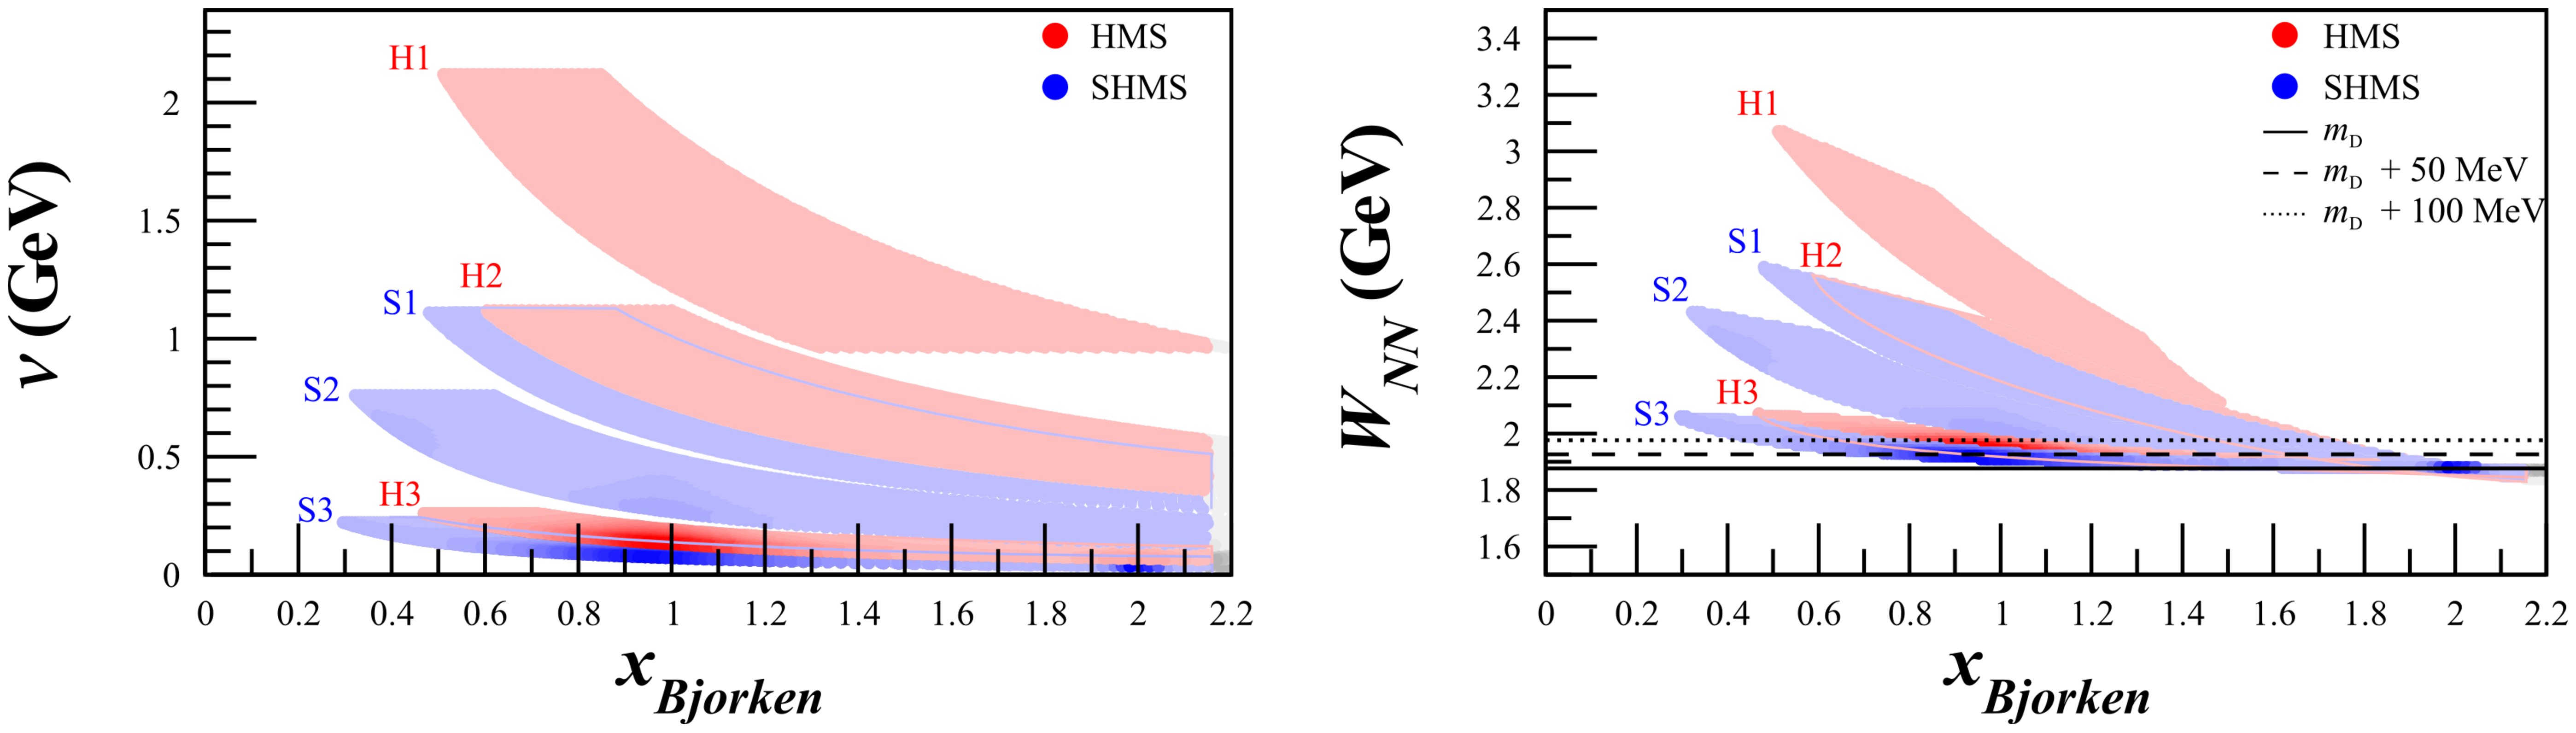
\includegraphics[width=\textwidth]{figs/Pzz_30_all_nu_wnn.eps}
%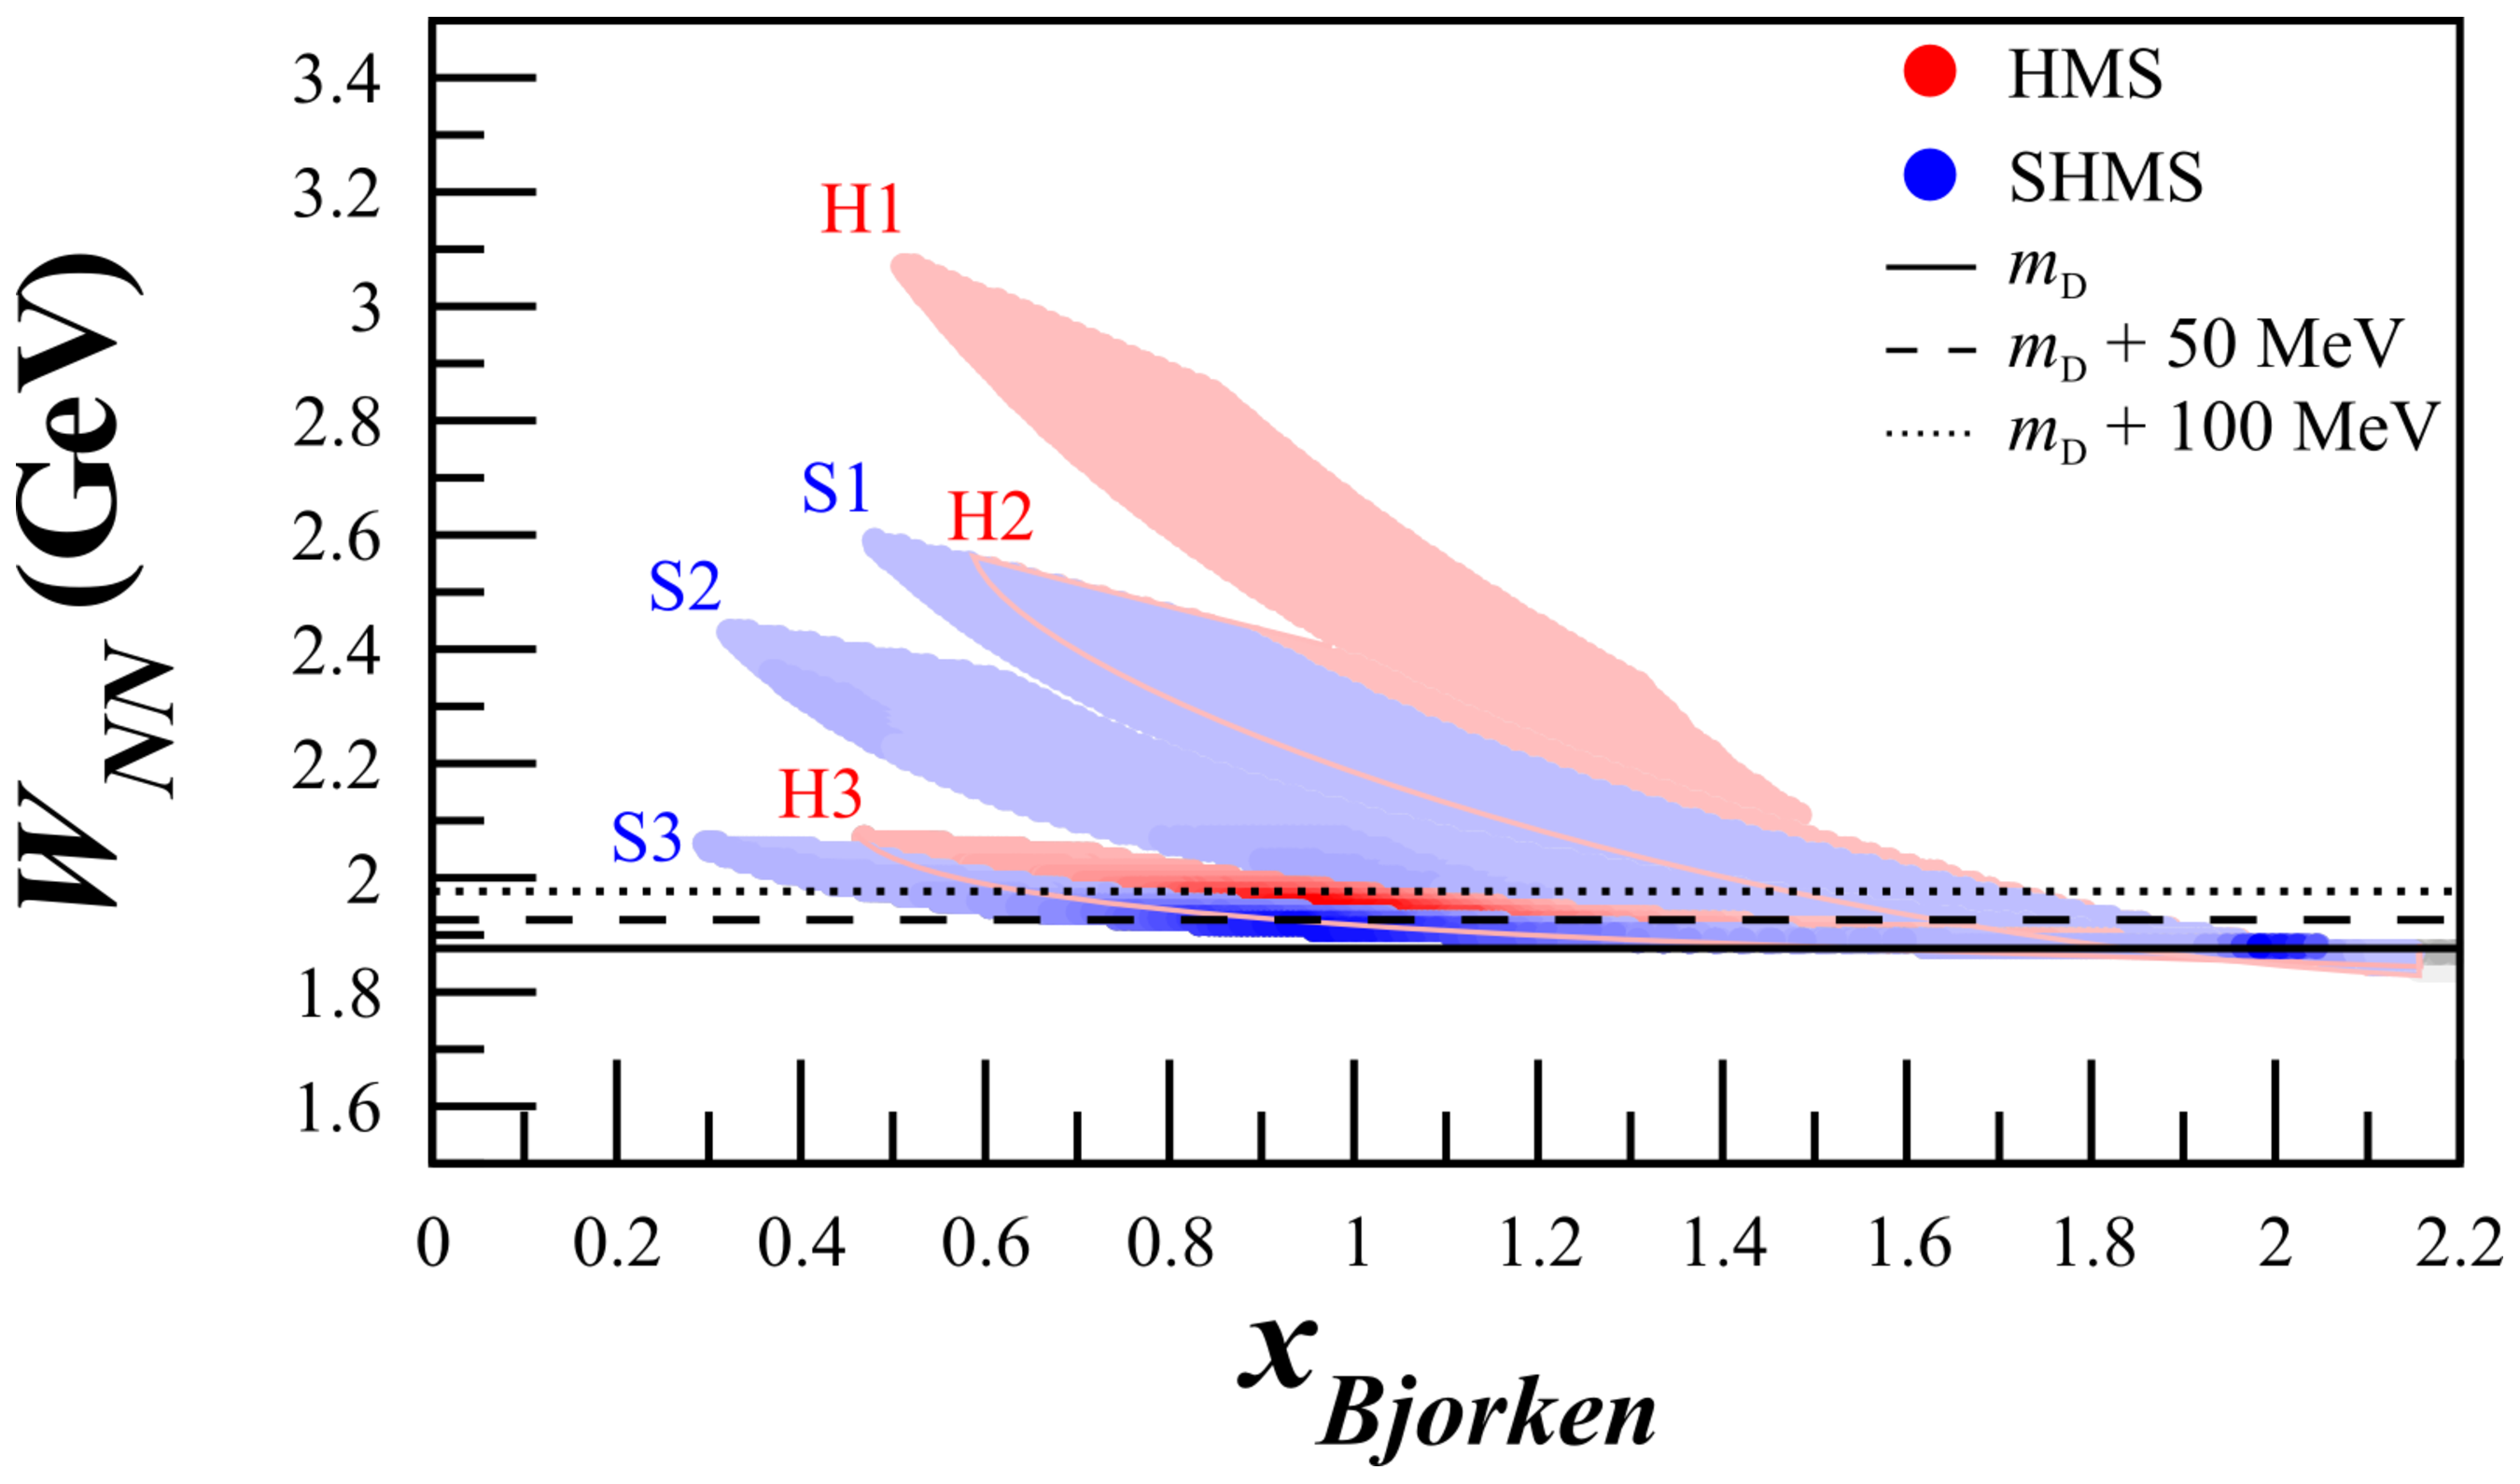
\includegraphics[width=0.49\textwidth]{figs/Pzz_30_all_wnn.eps} %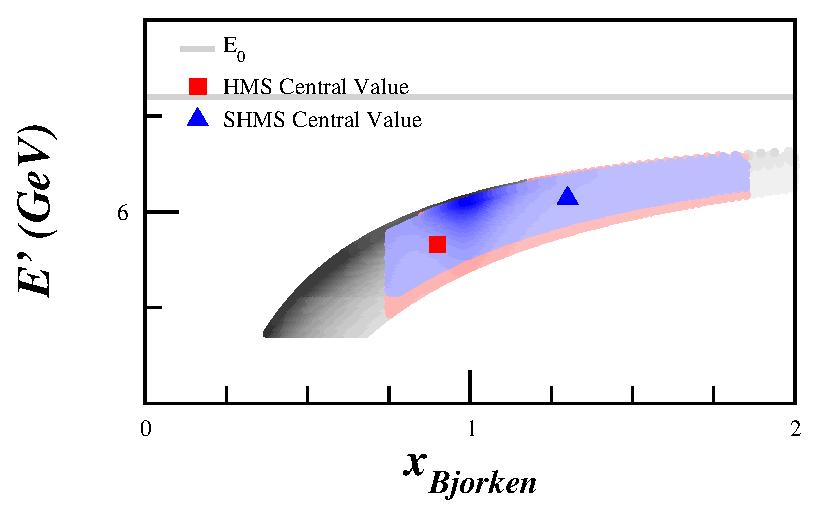
\includegraphics[width=0.49\textwidth]{figs/kine/Pzz_30_eprime.eps}
%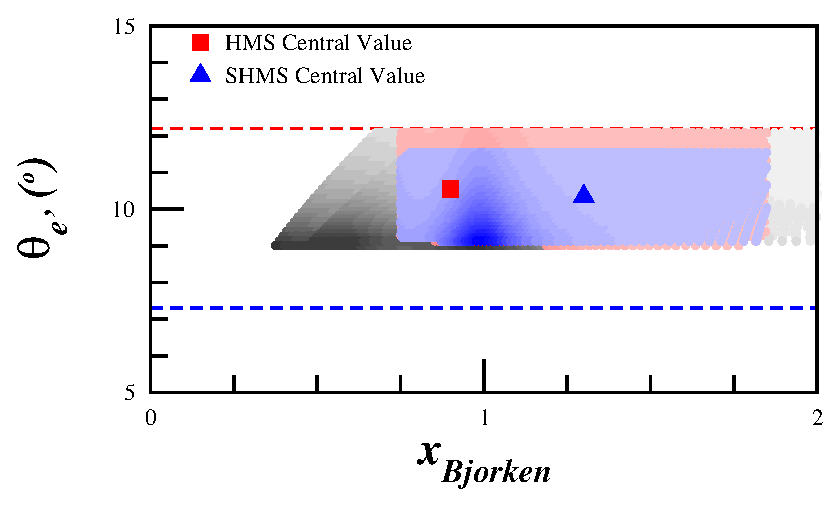
\includegraphics[width=0.49\textwidth]{figs/kine/Pzz_30_theta_eprime.eps}~~ 

\caption{\label{kincov} Kinematic coverage for central spectrometer settings at $Q^2=2.9~(\mathrm{GeV}/c)^2$ (H1), $1.8~(\mathrm{GeV}/c)^2$ (H2), $1.5~(\mathrm{GeV}/c)^2$ (S1), $0.7~(\mathrm{GeV}/c)^2$ (S2), $0.3~(\mathrm{GeV}/c)^2$ (H3), and $0.2~(\mathrm{GeV}/c)^2$ (S3). The grey regions are not included in our statistics estimates since they fall outside the range of electron-deuteron scattering. Darker shading represents areas with higher statistics. The solid, dashed, and dotted lines in the $W_{NN}$ plot indicate deuteron mass, deuteron mass + 50 MeV, and deuteron mass + 100 MeV, respectively. Virtual-nucleon and light cone calculations are only valid for $W_{NN}>m_D+50$~MeV.}
\end{center}
\end{figure}


The polarized \TARGET target is discussed in Section~\ref{POLTARGSEC}.  The magnetic field of the target will be held constant along the beamline at all times, while the target state is alternated between a polarized and unpolarized state.
The tensor polarization and packing fraction used in the rates estimate are \PZZ\% and \PF, respectively. 
The dilution factor in the range of this measurement is shown in Fig.~\ref{fdil_plot}. The spread of the elastic peak for the dilution factor was calculated assuming a momentum resolution of $0.1\%$ for the HMS and $0.08\%$ for the SHMS.
With an incident electron beam current of \CURRENT nA, the expected deuteron luminosity is \LUMI.
%$1.57\times 10^{35}$~cm$^{-2}}$s$^{-1}$.
%$?.??\times 10^{35}$~cm$^{-2}$s$^{-1}$.

\begin{figure}
\begin{center}
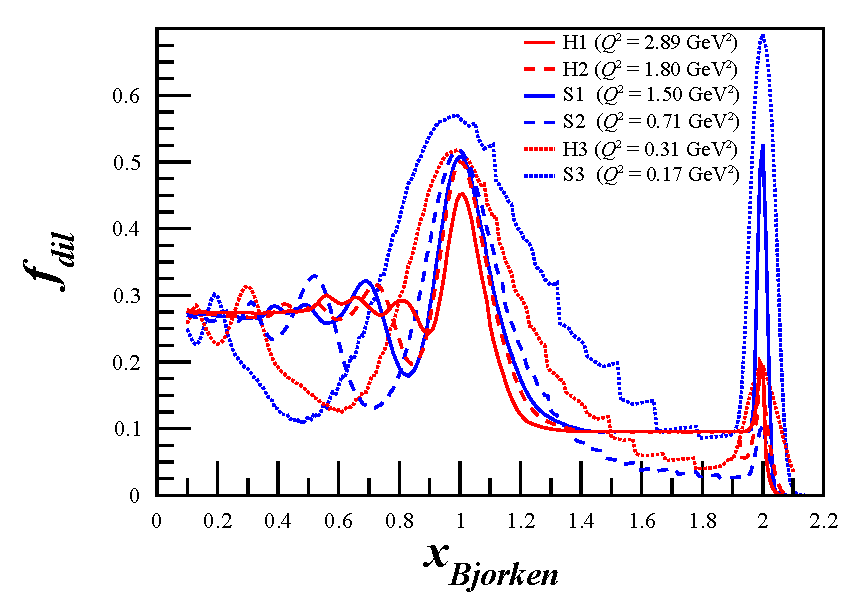
\includegraphics[width=0.65\textwidth]{figs/Pzz_30_fdil_all.eps} 
\caption{\label{fdil_plot}Projected dilution factor covering the entire $x$ range to be measured using a combination of P. Bosted's~\cite{Bosted:2012qc} and M. Sargsian's~\cite{misak-convo} code, along with a calculation of the elastic peak using a parametrization of the deuteron form factors, for the SHMS and HMS.}
\end{center}
\end{figure}


The momentum bite and the acceptance were assumed to be $\Delta P = \pm 8\%$ and $\Delta\Omega = 5.6$~msr for the HMS, and $\Delta P= ^{+20\%}_{-8\%}$ 
%$-8<\Delta P <+20\%$
and $\Delta\Omega =4.4$~msr for the SHMS. 
%
For the choice of the kinematics,
special attention was taken onto the angular and momentum limits of the spectrometers with a longitudinal polarized target: for the
HMS, $12.2^{\circ} \le \theta \le 85^{\circ}$ and $1 \le P_0 \le 7.3$ GeV/c, and for the SHMS,
$5.5^{\circ} \le \theta \le 40^{\circ}$ and $2 \le P_0 \le 11$ GeV/c. In addition, the
opening angle between the spectrometers is physically constrained to be larger than 17.5$^{\circ}$.

A total of \productiondays days of beam time is requested for production data, with an additional \overheaddays days of expected overhead.



\clearpage

%





